\documentclass[tikz]{standalone}
\usepackage{pgfplots}
\pgfplotsset{compat=1.15}
\usepackage{mathrsfs}
\usetikzlibrary{arrows,calc}
\usepackage{tkz-euclide}
\pagestyle{empty}

\definecolor{AngleClr}{rgb}{0,0.39215686274509803,0}
\definecolor{ShapeClr}{rgb}{0.6,0.2,0}

\begin{document}

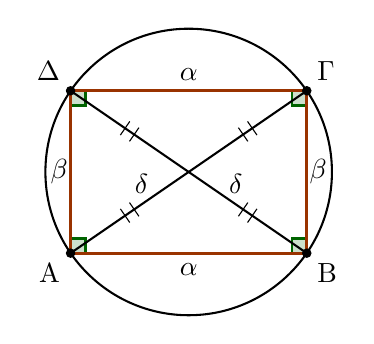
\begin{tikzpicture}[scale=.75]
\tkzSetUpLine[line width=1pt,color=black]
\tkzSetUpPoint[fill=black]

\tkzDefPoints{0/0/A,4/0/B,0/2.75/D,4/2.75/C}

\tkzDefMidPoint(A,C) \tkzGetPoint{O}


\tkzFillPolygon[fill=white](A,B,C,D)

\tkzMarkRightAngles[line width=1pt, size=.25,color=AngleClr,fill=AngleClr,fill opacity=0.2](A,B,C B,C,D C,D,A D,A,B)
\tkzDrawSegments[line width=0.75pt,color=black](A,C B,D)

\tkzDrawCircle[line width=0.75pt,color=black](O,A)

\tkzDrawPolygon[color=ShapeClr](A,B,C,D)
\tkzDrawPoints[size=3](A,B,C,D)
\tkzLabelPoint[below left](A){$\rm A$}
\tkzLabelPoint[below right](B){$\rm B$}
\tkzLabelPoint[above right](C){$\rm \Gamma$};
\tkzLabelPoint[above left](D){$\rm \Delta$};

\tkzMarkSegments[mark=||,size=3](O,A O,B O,C O,D)

\tkzLabelSegments[below](A,B){$\alpha$}
\tkzLabelSegments[right=-0.1cm](B,C){$\beta$}
\tkzLabelSegments[above](C,D){$\alpha$}
\tkzLabelSegments[left=-0.1cm](D,A){$\beta$}

\tkzLabelSegments[above,pos=0.3](A,C){$\delta$}
\tkzLabelSegments[above,pos=0.3](B,D){$\delta$}


\end{tikzpicture}

\end{document}
